
\documentclass[aspectratio=169,9pt]{beamer}

\usepackage[utf8]{inputenc}
\usepackage[T1]{fontenc}
\usepackage{lmodern}
\usepackage{microtype}
\usepackage{graphicx}
\usepackage{booktabs}
\usepackage{array}
\usepackage{amsmath}
\usepackage{pgfplots}
\usepackage{tikz}
\usepackage{ragged2e}
\usepackage{etoolbox}

\usetikzlibrary{arrows.meta,calc,positioning,fit,shapes.geometric,backgrounds}
\pgfplotsset{compat=1.18}

\usetheme{default}
\usefonttheme{professionalfonts}
\setbeamertemplate{navigation symbols}{}
\setbeamersize{text margin left=0.45cm,text margin right=0.45cm}

\definecolor{night}{HTML}{F7FAFC}
\definecolor{panel}{HTML}{FFFFFF}
\definecolor{panelsoft}{HTML}{EAF2FF}
\definecolor{panelline}{HTML}{A9BCD8}
\definecolor{textmain}{HTML}{10233D}
\definecolor{textmuted}{HTML}{5F7592}
\definecolor{accent}{HTML}{1783E7}
\definecolor{accentdeep}{HTML}{0F4FBF}
\definecolor{accentsoft}{HTML}{3A6EA5}
\definecolor{good}{HTML}{159A6F}
\definecolor{warn}{HTML}{C98A18}
\definecolor{bad}{HTML}{D96666}

\setbeamercolor{background canvas}{bg=night}
\setbeamercolor{normal text}{fg=textmain,bg=night}
\setbeamercolor{frametitle}{fg=textmain,bg=panelsoft}
\setbeamercolor{block title}{fg=textmain,bg=panelsoft}
\setbeamercolor{block body}{fg=textmain,bg=panel}
\setbeamercolor{title}{fg=textmain}
\setbeamercolor{subtitle}{fg=accentsoft}

\setbeamertemplate{itemize item}{\color{accent}\raisebox{0.15ex}{\tiny$\blacktriangleright$}}
\setbeamertemplate{itemize subitem}{\color{accent}\tiny$\bullet$}

\setbeamertemplate{frametitle}{
  \vspace*{0.15cm}
  \hspace*{0.10cm}
  \begin{beamercolorbox}[wd=\dimexpr\paperwidth-0.75cm\relax,ht=2.7ex,dp=0.9ex,rounded=true,leftskip=0.42cm]{frametitle}
    \usebeamerfont{frametitle}\insertframetitle
  \end{beamercolorbox}
}

\setbeamertemplate{footline}{}

\newcommand{\astrobackground}{
  \begin{tikzpicture}[remember picture,overlay]
    \fill[night] (current page.south west) rectangle (current page.north east);
    \fill[accent!12] ($(current page.north east)+(-1.8,-1.4)$) circle[radius=3.1cm];
    \fill[accentdeep!8] ($(current page.south east)+(-1.4,1.2)$) circle[radius=2.4cm];
    \draw[panelline, line width=0.35pt, opacity=0.65] ($(current page.south east)+(-2.0,1.3)$) circle[radius=1.9cm];
    \draw[panelline, line width=0.35pt, opacity=0.45] ($(current page.south east)+(-2.0,1.3)$) circle[radius=2.7cm];
    \fill[accentdeep] ($(current page.south east)+(-0.4,1.3)$) circle[radius=0.10cm];
    \fill[good] ($(current page.south east)+(-4.1,1.3)$) circle[radius=0.08cm];
    \foreach \x/\y/\r in {
      0.8/6.7/0.025, 1.6/5.8/0.020, 2.9/7.1/0.026, 4.2/6.4/0.018,
      5.8/7.5/0.030, 7.3/6.2/0.018, 8.9/7.3/0.022, 10.3/6.0/0.016,
      12.0/7.0/0.024, 13.5/6.4/0.018, 14.9/7.2/0.020, 2.1/3.9/0.015,
      5.0/4.2/0.018, 8.2/3.7/0.015, 11.6/4.0/0.017, 13.8/4.6/0.015
    }{
      \fill[accentdeep!55] ($(current page.south west)+(\x,\y)$) circle[radius=\r];
    }
  \end{tikzpicture}
}

\newcommand{\phasebar}[1]{
  \begin{beamercolorbox}[wd=\linewidth,sep=0.22em,rounded=true]{block body}
    {\scriptsize\color{accent}\bfseries CRISP-DM \hspace{0.6em}\color{textmuted}#1}
  \end{beamercolorbox}
}

\newcommand{\metriccard}[3]{
  \begin{beamercolorbox}[wd=\linewidth,sep=0.38em,rounded=true]{block body}
    {\scriptsize\color{textmuted}#1}\par
    \vspace{0.04em}
    {\fontsize{16}{17}\selectfont\bfseries #2}\par
    \vspace{0.08em}
    {\scriptsize #3}
  \end{beamercolorbox}
}

\newcommand{\infocard}[2]{
  \begin{beamercolorbox}[wd=\linewidth,sep=0.34em,rounded=true]{block body}
    {\small\bfseries #1}\par
    \vspace{0.05em}
    {\scriptsize #2}
  \end{beamercolorbox}
}

\newcommand{\closingbanner}[1]{
  \begin{beamercolorbox}[wd=\linewidth,sep=0.85em,rounded=true]{block title}
    \centering{\Large\bfseries #1}
  \end{beamercolorbox}
}

\newcommand{\badge}[2]{%
  \fcolorbox{#1}{panelsoft}{\textcolor{textmain}{\scriptsize\strut\hspace{0.30em}#2\hspace{0.30em}}}%
}

\newcommand{\rankbar}[4]{%
  {\scriptsize\color{textmain}#2\hfill #3}\par
  \begin{tikzpicture}
    \fill[panelsoft] (0,0) rectangle (4.75,0.17);
    \pgfmathsetmacro{\barw}{4.75*(#4)}
    \fill[#1] (0,0) rectangle (\barw,0.18);
  \end{tikzpicture}\par
  \vspace{0.03cm}
}

\newcommand{\safeincludegraphics}[2][]{%
  \IfFileExists{#2}{%
    \includegraphics[#1]{#2}%
  }{%
    \begin{tikzpicture}
      \node[draw=panelline,rounded corners=5pt,fill=panel,minimum width=0.94\linewidth,minimum height=0.28\textheight,align=center,text width=0.82\linewidth] {\scriptsize Figura no disponible\\\texttt{#2}};
    \end{tikzpicture}%
  }%
}

\begin{document}

\begin{frame}[plain,noframenumbering]
  \astrobackground
  \vspace*{0.45cm}
  {\color{accent}\normalsize\bfseries EXODATA UDLAP}\par
  \vspace{0.32cm}
  {\fontsize{23}{25}\selectfont\bfseries Topolog\'ia del universo observable}\\[0.05cm]
  {\fontsize{23}{25}\selectfont\bfseries de exoplanetas}\par
  \vspace{0.24cm}
  {\normalsize\color{accentsoft}De sesgos de detecci\'on a regiones observacionalmente informativas}\par
  \vspace{0.42cm}
  \begin{columns}[T,onlytextwidth]
    \begin{column}{0.58\textwidth}
      \begin{beamercolorbox}[wd=\linewidth,sep=0.82em,rounded=true]{block body}
        {\small\bfseries Tesis del proyecto}\par
        \vspace{0.12em}
        {\small El cat\'alogo NASA no representa el universo real de planetas. Representa el universo observable: lo que instrumentos, m\'etodos e historia observacional han permitido registrar.}\\[0.18cm]
        {\small\color{textmuted}Fuente}\par
        {\large NASA Exoplanet Archive -- \texttt{PSCompPars}}\\
        {\small 6273 exoplanetas}
      \end{beamercolorbox}
    \end{column}
    \begin{column}{0.37\textwidth}
      \begin{beamercolorbox}[wd=\linewidth,sep=0.70em,rounded=true]{block body}
        {\small\bfseries Entrega t\'ecnica}\par
        \vspace{0.10em}
        {\small Mapper/TDA}\\[0.03cm]
        {\small auditor\'ia observacional}\\[0.03cm]
        {\small Shadow Score}\\[0.03cm]
        {\small TOI y ATI}\\[0.03cm]
        {\small gaps intra-sistema alrededor de estrellas}
      \end{beamercolorbox}
    \end{column}
  \end{columns}
  \vspace{0.28cm}
  {\small\color{textmuted}21 gr\'aficas Mapper | PCA2 principal | DBSCAN local | ranking global y extensi\'on a sistemas planetarios}
\end{frame}

\begin{frame}[t,shrink=2]{Idea central: universo real vs universo observable}
  \phasebar{1. Business Understanding}
  \vspace{0.12cm}
  \begin{columns}[T,onlytextwidth]
    \begin{column}{0.46\textwidth}
      \begin{beamercolorbox}[wd=\linewidth,sep=0.80em,rounded=true]{block body}
        {\Large\bfseries ``No observamos todos los planetas.''}\\[0.12cm]
        {\Large\bfseries ``Observamos los que podemos detectar.''}
      \end{beamercolorbox}
      \vspace{0.12cm}
      \infocard{Problema cient\'ifico}{El cat\'alogo mezcla se\~nal astrof\'isica con l\'imites instrumentales, geometr\'ia de detecci\'on, m\'etodos de descubrimiento y selecci\'on humana de targets.}
    \end{column}
    \begin{column}{0.51\textwidth}
      \begin{center}
        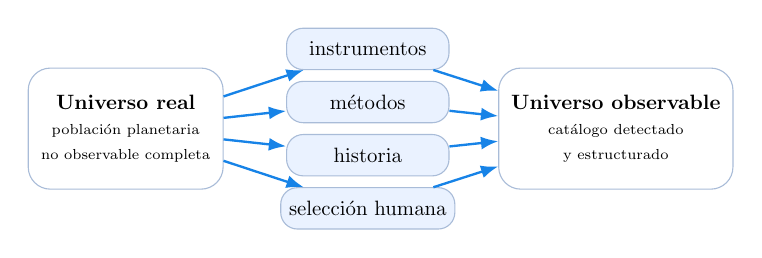
\begin{tikzpicture}[scale=0.75,transform shape,
          box/.style={rounded corners=8pt, draw=panelline, fill=panel, minimum width=3.3cm, minimum height=1.45cm, align=center, inner sep=6pt},
          filter/.style={rounded corners=6pt, draw=panelline, fill=panelsoft, minimum width=2.75cm, minimum height=0.70cm, align=center, inner sep=4pt},
          arrow/.style={-{Latex[length=2.2mm]}, line width=0.85pt, color=accent}
        ]
          \node[box, minimum height=2.05cm] (real) at (0,0) {\textbf{Universo real}\\\scriptsize poblaci\'on planetaria\\\scriptsize no observable completa};
          \node[filter] (inst) at (4.1,1.35) {instrumentos};
          \node[filter] (meth) at (4.1,0.45) {m\'etodos};
          \node[filter] (hist) at (4.1,-0.45) {historia};
          \node[filter] (human) at (4.1,-1.35) {selecci\'on humana};
          \node[box, minimum height=2.05cm] (obs) at (8.3,0) {\textbf{Universo observable}\\\scriptsize cat\'alogo detectado\\\scriptsize y estructurado};
          \draw[arrow] (real) -- (inst);
          \draw[arrow] (real) -- (meth);
          \draw[arrow] (real) -- (hist);
          \draw[arrow] (real) -- (human);
          \draw[arrow] (inst) -- (obs);
          \draw[arrow] (meth) -- (obs);
          \draw[arrow] (hist) -- (obs);
          \draw[arrow] (human) -- (obs);
        \end{tikzpicture}
      \end{center}
      \vspace{0.05cm}
      \closingbanner{La pregunta no es solo qu\'e planetas hay; es qu\'e planetas logramos ver.}
    \end{column}
  \end{columns}
\end{frame}

\begin{frame}[t,shrink=2]{Metodolog\'ia CRISP-DM}
  \phasebar{1--6. Del problema a comunicaci\'on}
  \vspace{0.10cm}
  \begin{center}
    
\begin{tikzpicture}[
      stage/.style={draw=panelline,fill=panel,rounded corners=7pt,minimum width=2.34cm,minimum height=1.08cm,align=center,font=\scriptsize,text width=2.12cm},
      arrow/.style={-{Latex[length=2.1mm]},line width=0.8pt,color=accent}
    ]
      \node[stage] (b) at (0,0) {\textbf{Business}\\universo observable};
      \node[stage] (d) at (2.55,0) {\textbf{Data}\\NASA PSCompPars};
      \node[stage] (p) at (5.10,0) {\textbf{Preparation}\\log, scaling, imputaci\'on};
      \node[stage] (m) at (7.65,0) {\textbf{Modeling}\\Mapper/TDA};
      \node[stage] (e) at (10.20,0) {\textbf{Evaluation}\\topolog\'ia + sesgo};
      \node[stage] (c) at (12.75,0) {\textbf{Communication}\\prioridades};
      \draw[arrow] (b)--(d);
      \draw[arrow] (d)--(p);
      \draw[arrow] (p)--(m);
      \draw[arrow] (m)--(e);
      \draw[arrow] (e)--(c);
    \end{tikzpicture}
  \end{center}
  \vspace{0.18cm}
  \begin{columns}[T,onlytextwidth]
    \begin{column}{0.32\textwidth}
      \infocard{ 1: cat\'alogo}{Construimos un mapa topol\'ogico global del universo observable.}
    \end{column}
    \begin{column}{0.32\textwidth}
      \infocard{ 2: regiones}{Convertimos fronteras observacionales en TOI y ATI.}
    \end{column}
    \begin{column}{0.32\textwidth}
      \infocard{ 3: estrellas}{Trasladamos la se\~nal global a gaps orbitales dentro de sistemas conocidos.}
    \end{column}
  \end{columns}
  \vspace{0.12cm}
  \closingbanner{El proyecto no termina en una gr\'afica: termina en preguntas observacionales accionables.}
\end{frame}

\begin{frame}[t,shrink=8]{Datos y preparaci\'on}
  \phasebar{2--3. Data Understanding y Preparation}
  \vspace{0.06cm}
  \begin{columns}[T,onlytextwidth]
    \begin{column}{0.48\textwidth}
      \infocard{Variables planetarias}{Bloques f\'isico, orbital y t\'ermico: masa, radio, densidad, per\'iodo orbital, semieje mayor, insolaci\'on y temperatura de equilibrio.}
      \vspace{0.05cm}
      \infocard{Trazabilidad}{Observado = medido. Derivado = calculado. Imputado = completado por el pipeline. La imputaci\'on preserva continuidad anal\'itica, pero no agrega evidencia nueva.}
      \vspace{0.05cm}
      \infocard{Lectura prudente}{No tratamos imputaci\'on y dato medido como equivalentes. Si un nodo depende mucho de imputaci\'on, la geometr\'ia puede mantenerse, pero baja su fuerza interpretativa.}
    \end{column}
    \begin{column}{0.48\textwidth}
      \begin{beamercolorbox}[wd=\linewidth,sep=0.42em,rounded=true]{block body}
        {\small\bfseries Auditor\'ia de datos}
      \end{beamercolorbox}
      \vspace{0.04cm}
      \safeincludegraphics[width=\linewidth,height=0.34\textheight,keepaspectratio]{figures/02_value_source_composition.pdf}
      \vspace{0.04cm}
      \infocard{Metadata observacional}{\texttt{discoverymethod}, a\~no y facility se reservan para auditor\'ia; no construyen directamente la geometr\'ia principal.}
    \end{column}
  \end{columns}
  \vspace{0.05cm}
  \begin{columns}[T,onlytextwidth]
    \begin{column}{0.25\textwidth}
      \metriccard{Espacios}{7}{f\'isico, orbital, t\'ermico y combinados}
    \end{column}
    \begin{column}{0.25\textwidth}
      \metriccard{Estados}{3}{observado, derivado, imputado}
    \end{column}
    \begin{column}{0.25\textwidth}
      \metriccard{Auditor\'ia}{externa}{el sesgo no entra al lente}
    \end{column}
    \begin{column}{0.25\textwidth}
      \metriccard{Regla}{cautela}{si sube imputaci\'on, baja confianza}
    \end{column}
  \end{columns}
\end{frame}

\begin{frame}[t,shrink=5]{Por qu\'e Mapper como modelado no supervisado}
  \phasebar{4. Modeling}
  \vspace{0.06cm}
  \begin{columns}[T,onlytextwidth]
    \begin{column}{0.48\textwidth}
      \infocard{No impone clases fijas}{No exige fijar cu\'antos grupos existen antes de mirar la geometr\'ia.}
      \vspace{0.05cm}
      \infocard{Conserva continuidad}{Nos interesan transiciones, periferias y puentes, no solo clusters compactos.}
      \vspace{0.05cm}
      \infocard{Tolera geometr\'ias complejas}{Resume espacios no convexos y vecindarios que se superponen.}
      \vspace{0.05cm}
      \infocard{Es auditable}{Cada nodo puede revisarse por m\'etodo, imputaci\'on, tama\~no y coherencia f\'isica local.}
    \end{column}
    \begin{column}{0.48\textwidth}
      \begin{beamercolorbox}[wd=\linewidth,sep=0.42em,rounded=true]{block body}
        {\small\bfseries Especificaci\'on del experimento Mapper}\par
        \vspace{0.04cm}
        \[
        7\ \text{espacios}\times 3\ \text{lentes}=21\ \text{grafos}
        \]
        {\scriptsize Espacios: f\'isico, orbital, t\'ermico y combinados.}\par
        \vspace{0.04cm}
        {\scriptsize Lente principal: PCA2. Sensibilidad: \texttt{domain} y \texttt{density}.}\par
        \vspace{0.04cm}
        {\scriptsize Cover fijo: 10 cubos con \texttt{overlap = 0.35}. Clustering local: DBSCAN.}
      \end{beamercolorbox}
      \vspace{0.06cm}
      \begin{beamercolorbox}[wd=\linewidth,sep=0.42em,rounded=true]{block body}
        {\small\bfseries Lectura metodol\'ogica}\par
        \vspace{0.05cm}
        {\scriptsize Mapper funciona aqu\'i como aprendizaje no supervisado orientado a forma: resume geometr\'ia y luego deja auditar si esa forma refleja estructura planetaria, sesgo observacional o mezcla de ambos.}
      \end{beamercolorbox}
    \end{column}
  \end{columns}
  \vspace{0.12cm}
  \closingbanner{Usamos Mapper para conservar forma observable, no para forzar una taxonom\'ia cerrada.}
\end{frame}

\begin{frame}[t]{C\'omo funciona Mapper paso a paso}
  \phasebar{4. Modeling}
  \vspace{0.10cm}
  \begin{columns}[T,onlytextwidth]
    \begin{column}{0.24\textwidth}
      \infocard{1. Lente}{PCA2 proyecta el espacio para observar gradientes globales.}
      \vspace{0.08cm}
      \begin{tikzpicture}[scale=0.72]
        \fill[panel] (0,0) rectangle (4.5,2.8);
        \foreach \x/\y in {0.5/0.5,0.9/0.8,1.2/1.4,1.7/1.2,2.1/1.8,2.5/1.4,2.9/2.1,3.3/1.8,3.8/2.4,2.6/0.8,3.4/0.9}{
          \fill[accent] (\x,\y) circle[radius=0.06];
        }
        \draw[->,color=textmuted] (0.4,0.35)--(4.2,0.35);
        \draw[->,color=textmuted] (0.4,0.35)--(0.4,2.55);
      \end{tikzpicture}
    \end{column}
    \begin{column}{0.24\textwidth}
      \infocard{2. Cover}{Vecindarios solapados: 10 cubos y overlap 0.35.}
      \vspace{0.08cm}
      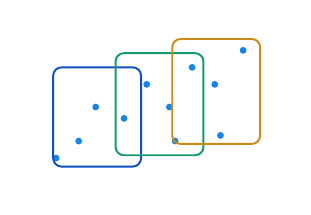
\begin{tikzpicture}[scale=0.72]
        \fill[panel] (0,0) rectangle (4.5,2.8);
        \foreach \x/\y in {0.5/0.5,0.9/0.8,1.2/1.4,1.7/1.2,2.1/1.8,2.5/1.4,2.9/2.1,3.3/1.8,3.8/2.4,2.6/0.8,3.4/0.9}{
          \fill[accent] (\x,\y) circle[radius=0.06];
        }
        \draw[accentdeep,line width=0.7pt,rounded corners=3pt] (0.45,0.35) rectangle (2.0,2.1);
        \draw[good,line width=0.7pt,rounded corners=3pt] (1.55,0.55) rectangle (3.10,2.35);
        \draw[warn,line width=0.7pt,rounded corners=3pt] (2.55,0.75) rectangle (4.10,2.60);
      \end{tikzpicture}
    \end{column}
    \begin{column}{0.24\textwidth}
      \infocard{3. DBSCAN}{Clustering local sin imponer un n\'umero fijo de grupos.}
      \vspace{0.08cm}
      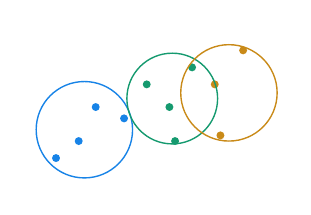
\begin{tikzpicture}[scale=0.72]
        \fill[panel] (0,0) rectangle (4.5,2.8);
        \foreach \x/\y/\c in {0.5/0.5/accent,0.9/0.8/accent,1.2/1.4/accent,1.7/1.2/accent,2.1/1.8/good,2.5/1.4/good,2.9/2.1/good,3.3/1.8/warn,3.8/2.4/warn,2.6/0.8/good,3.4/0.9/warn}{
          \fill[\c] (\x,\y) circle[radius=0.07];
        }
        \draw[accent,line width=0.5pt] (1.0,1.0) circle[radius=0.85];
        \draw[good,line width=0.5pt] (2.55,1.55) circle[radius=0.80];
        \draw[warn,line width=0.5pt] (3.55,1.65) circle[radius=0.85];
      \end{tikzpicture}
    \end{column}
    \begin{column}{0.24\textwidth}
      \infocard{4. Grafo}{Nodo = comunidad local. Arista = solapamiento de miembros.}
      \vspace{0.08cm}
      \safeincludegraphics[width=\linewidth,height=0.25\textheight,keepaspectratio]{figures/orbital_graph_discoverymethod.pdf}
    \end{column}
  \end{columns}
  \vspace{0.14cm}
  \closingbanner{Mapper conserva continuidad, periferias y transiciones: justo lo que necesitamos para leer sesgo observacional.}
\end{frame}



\begin{frame}[t]{Qu\'e representa el grafo en esta historia}
  \phasebar{4. Modeling}
  \vspace{0.10cm}
  \safeincludegraphics[width=\linewidth,height=0.47\textheight,keepaspectratio]{figures/astro_orbital_graph_by_orbit_class.pdf}
  \vspace{0.08cm}
  \begin{columns}[T,onlytextwidth]
    \begin{column}{0.24\textwidth}
      \infocard{Nodo denso}{Zona altamente observable o muy poblada dentro del cat\'alogo.}
    \end{column}
    \begin{column}{0.24\textwidth}
      \infocard{Rama}{R\'egimen especializado: puede mezclar f\'isica y m\'etodo de detecci\'on.}
    \end{column}
    \begin{column}{0.24\textwidth}
      \infocard{Puente}{Transici\'on entre reg\'imenes orbitales u observacionales.}
    \end{column}
    \begin{column}{0.24\textwidth}
      \infocard{Hueco}{Baja cobertura relativa: candidato para inspecci\'on, no prueba de ausencia.}
    \end{column}
  \end{columns}
\end{frame}

\begin{frame}[t,shrink=4]{Conclusi\'on intermedia: el Mapper orbital s\'i organiza sesgo observacional}
  \phasebar{5. Evaluation}
  \vspace{0.10cm}
  \begin{columns}[T,onlytextwidth]
    \begin{column}{0.58\textwidth}
      \safeincludegraphics[width=\linewidth,height=0.49\textheight,keepaspectratio]{figures/orbital_graph_discoverymethod.pdf}
      \vspace{0.06cm}
      \infocard{Lectura}{El grafo orbital no solo organiza vecindades planetarias. Tambi\'en conserva informaci\'on sobre c\'omo fueron descubiertos esos planetas.}
    \end{column}
    \begin{column}{0.38\textwidth}
      \begin{columns}[T,onlytextwidth]
        \begin{column}{0.50\textwidth}
          \metriccard{NMI}{0.165}{nodo vs. m\'etodo}
        \end{column}
        \begin{column}{0.50\textwidth}
          \metriccard{z}{138.9}{muy lejos del nulo}
        \end{column}
      \end{columns}
      \vspace{0.08cm}
      \metriccard{p}{0.001}{asociaci\'on significativa}
      \vspace{0.08cm}
      \infocard{Conclusi\'on}{Existe sesgo observacional estructurado en los nodos del Mapper. Eso no invalida el mapa; explica por qu\'e necesitamos auditarlo antes de priorizar.}
      \vspace{0.08cm}
      \infocard{Paso siguiente}{Shadow Score, TOI y ATI convierten esa huella observacional en una prioridad local y regional interpretable.}
    \end{column}
  \end{columns}
\end{frame}

\begin{frame}[t,shrink=3]{Complejidad topol\'ogica del mapa: 124 nodos, 196 aristas, 96 ciclos independientes}
  \phasebar{5. Evaluation}
  \vspace{0.10cm}
  \begin{columns}[T,onlytextwidth]
    \begin{column}{0.63\textwidth}
      \safeincludegraphics[width=\linewidth,height=0.58\textheight,keepaspectratio]{figures/01_mapper_graph_size_complexity.pdf}
    \end{column}
    \begin{column}{0.33\textwidth}
      \infocard{Lectura}{No buscamos solo complejidad visual. Buscamos una geometr\'ia interpretable y metodol\'ogicamente defendible.}
      \vspace{0.08cm}
      \infocard{M\'etricas}{Nodos, aristas y $\beta_1$ resumen riqueza topol\'ogica. La imputaci\'on media limita cu\'anto confiar en esa estructura.}
      \vspace{0.08cm}
      \infocard{Conclusi\'on}{El espacio orbital destaca porque conserva mucha estructura sin depender de imputaci\'on extensa.}
    \end{column}
  \end{columns}
\end{frame}

\begin{frame}[t,shrink=4]{Resultado global: el espacio orbital como mapa principal}
  \phasebar{5. Evaluation}
  \vspace{0.10cm}
  \begin{columns}[T,onlytextwidth]
    \begin{column}{0.60\textwidth}
      \safeincludegraphics[width=\linewidth,height=0.49\textheight,keepaspectratio]{figures/orbital_graph_imputation.pdf}
      \vspace{0.06cm}
      \infocard{Por qu\'e este mapa}{Alta complejidad + baja imputaci\'on = mapa defendible del universo observable orbital. La estructura no descansa principalmente en completaci\'on artificial del cat\'alogo y conserva trazabilidad razonable.}
    \end{column}
    \begin{column}{0.36\textwidth}
      \begin{columns}[T,onlytextwidth]
        \begin{column}{0.50\textwidth}
          \metriccard{Nodos}{124}{comunidades locales}
        \end{column}
        \begin{column}{0.50\textwidth}
          \metriccard{Aristas}{196}{continuidad topol\'ogica}
        \end{column}
      \end{columns}
      \vspace{0.08cm}
      \begin{columns}[T,onlytextwidth]
        \begin{column}{0.50\textwidth}
          \metriccard{$\beta_1$}{96}{ciclos independientes}
        \end{column}
        \begin{column}{0.50\textwidth}
          \metriccard{Imputaci\'on}{0.011}{dependencia baja}
        \end{column}
      \end{columns}
      \vspace{0.10cm}
      \infocard{Lectura prudente}{Baja imputaci\'on no significa verdad definitiva. Significa que, dentro del pipeline, este mapa requiere poca completaci\'on relativa para sostener su geometr\'ia y por eso admite una lectura m\'as fuerte.}
    \end{column}
  \end{columns}
\end{frame}

\begin{frame}[t]{Shadow Score: frontera observacional local}
  \phasebar{5--6. Evaluation y Communication}
  \vspace{0.08cm}
  \begin{columns}[T,onlytextwidth]
    \begin{column}{0.54\textwidth}
      \begin{beamercolorbox}[wd=\linewidth,sep=0.62em,rounded=true]{block body}
        {\small\bfseries Shadow Score = \'{\i}ndice local de frontera observacional}
        \[
        \mathrm{Shadow}(v)\propto f_{\mathrm{dom}}(v)(1-H(v))(1-I(v))B(v)S(v)
        \]
        {\scriptsize Crece cuando un nodo tiene m\'etodo dominante, baja entrop\'ia, baja imputaci\'on, contraste con vecinos y soporte suficiente. Resume una frontera local de cobertura observacional.}
      \end{beamercolorbox}
    \end{column}
    \begin{column}{0.42\textwidth}
      \infocard{Detecta}{cambios locales en cobertura observacional dentro del grafo.}
      \vspace{0.08cm}
      \infocard{No detecta}{planetas faltantes ni probabilidades f\'isicas de ausencia.}
      \vspace{0.08cm}
      \infocard{Caso orbital}{\texttt{cube17\_cluster2}: RV dominante, n=8, imputaci\'on 0.000, Shadow = 0.274.}
      \vspace{0.08cm}
      \infocard{Caso poblacional}{\texttt{cube51\_cluster1}: Transit dominante, n=79, imputaci\'on 0.000, Shadow = 0.552.}
    \end{column}
  \end{columns}
\end{frame}

\begin{frame}[t,shrink=8]{De mapa global a prioridad: TOI y ATI}
  \phasebar{6. Deployment / Communication}
  \vspace{0.01cm}
  \begin{columns}[T,onlytextwidth]
    \begin{column}{0.42\textwidth}
      \begin{beamercolorbox}[wd=\linewidth,sep=0.38em,rounded=true]{block body}
        {\small\bfseries Definici\'on regional}\par
        \[
        \resizebox{0.98\linewidth}{!}{$
        \mathrm{TOI}(v)=\mathrm{Shadow}(v)(1-I_{R^3}(v))C_{\mathrm{phys}}(v)S_{\mathrm{net}}(v)
        $}
        \]
        {\tiny Frontera observacional + baja imputaci\'on en \(R^3\) + coherencia f\'isica local + soporte de red.}
      \end{beamercolorbox}
      \vspace{0.05cm}
      \begin{beamercolorbox}[wd=\linewidth,sep=0.38em,rounded=true]{block body}
        {\small\bfseries Definici\'on por planeta ancla}\par
        \[
        \resizebox{0.98\linewidth}{!}{$
        \mathrm{ATI}(p^\ast)=\mathrm{TOI}(v)\Delta_{\mathrm{rel,best}}(p^\ast)(1-I_{R^3}(p^\ast))A(p^\ast)
        $}
        \]
        {\tiny Convierte una regi\'on prioritaria en un caso local: d\'eficit relativo, baja imputaci\'on y representatividad.}
      \end{beamercolorbox}
    \end{column}
    \begin{column}{0.54\textwidth}
      \begin{beamercolorbox}[wd=\linewidth,sep=0.32em,rounded=true]{block body}
        {\small\bfseries Top regiones por TOI}\par
        \vspace{0.02cm}
        \rankbar{accentdeep}{cube12\_cluster0}{0.07667}{1.00}
        \rankbar{accentdeep}{cube17\_cluster2}{0.06276}{0.82}
        \rankbar{accentdeep}{cube26\_cluster6}{0.05811}{0.76}
      \end{beamercolorbox}
      \vspace{0.04cm}
      \begin{beamercolorbox}[wd=\linewidth,sep=0.32em,rounded=true]{block body}
        {\small\bfseries Top planetas ancla por ATI conservador}\par
        \vspace{0.02cm}
        \rankbar{accent}{HIP 90988 b}{0.006389}{1.00}
        \rankbar{good}{HD 42012 b}{0.005113}{0.80}
        \rankbar{good}{HD 4313 b}{0.004348}{0.68}
      \end{beamercolorbox}
    \end{column}
  \end{columns}
  \vspace{0.03cm}
  \closingbanner{TOI prioriza nodos. ATI vuelve esa prioridad regional en un caso local auditable.}
\end{frame}

\begin{frame}[t,shrink=3]{El siguiente salto: de regiones globales a estrellas conocidas}
  \phasebar{6. Deployment / Communication}
  \vspace{0.04cm}
  \begin{columns}[T,onlytextwidth]
    \begin{column}{0.49\textwidth}
      \infocard{Antes}{El proyecto priorizaba regiones del cat\'alogo completo: nodos, fronteras y planetas ancla.}
      \vspace{0.08cm}
      \infocard{Ahora}{El m\'odulo \texttt{11\_stars} pregunta si esa se\~nal global puede traducirse a intervalos orbitales dentro de sistemas planetarios conocidos.}
      \vspace{0.08cm}
      \infocard{Nuevas variables}{Ahora trabajamos tambi\'en con propiedades estelares: \(M_\star\), \(R_\star\), arquitectura del sistema y m\'etodo dominante de descubrimiento.}
      \vspace{0.08cm}
      \infocard{Nueva unidad de salida}{Una estrella, dos planetas observados, un gap orbital, una posici\'on candidata y una raz\'on plausible de dificultad observacional.}
    \end{column}
    \begin{column}{0.47\textwidth}
      \begin{center}
        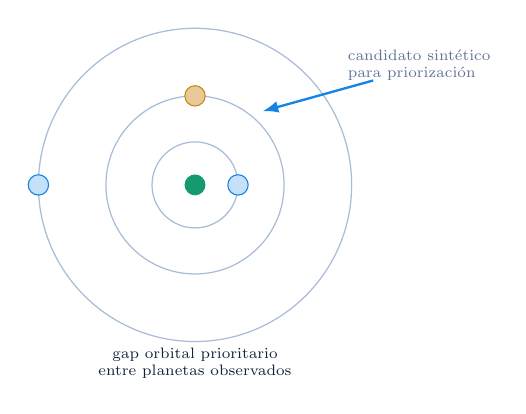
\begin{tikzpicture}[scale=0.78,transform shape,
          planet/.style={circle,draw=accent,fill=accent!25,minimum size=0.22cm},
          cand/.style={circle,draw=warn,fill=warn!45,minimum size=0.30cm},
          orbit/.style={draw=panelline,line width=0.45pt},
          arr/.style={-{Latex[length=2.0mm]},line width=0.85pt,color=accent}
        ]
          \fill[good] (0,0) circle[radius=0.17];
          \draw[orbit] (0,0) circle[radius=0.70];
          \draw[orbit] (0,0) circle[radius=1.45];
          \draw[orbit] (0,0) circle[radius=2.55];
          \node[planet] at (0.70,0) {};
          \node[cand] at (0,1.45) {};
          \node[planet] at (-2.55,0) {};
          \node[align=center,text=textmain,font=\scriptsize] at (0,-2.90) {gap orbital prioritario\\entre planetas observados};
          \draw[arr] (2.9,1.7) -- (1.1,1.2);
          \node[align=left,text=textmuted,font=\scriptsize] at (3.65,1.95) {candidato sint\'etico\\para priorizaci\'on};
        \end{tikzpicture}
      \end{center}
    \end{column}
  \end{columns}
\end{frame}

\begin{frame}[t,shrink=8]{Modelo intra-sistema: gaps orbitales con herencia topol\'ogica}
  \phasebar{4--5. Modeling y Evaluation}
  \vspace{0.04cm}
  \begin{columns}[T,onlytextwidth]
    \begin{column}{0.52\textwidth}
      \begin{beamercolorbox}[wd=\linewidth,sep=0.42em,rounded=true]{block body}
        {\small\bfseries Orden orbital observado}\par
        \[
          P_1 < P_2 < \cdots < P_n
        \]
        {\scriptsize \(P_i\) es el per\'iodo orbital de cada planeta observado. Cada par adyacente define un gap orbital.}
      \end{beamercolorbox}
      \vspace{0.06cm}
      \begin{beamercolorbox}[wd=\linewidth,sep=0.42em,rounded=true]{block body}
        {\small\bfseries Interpolaci\'on prudente, no imputaci\'on del cat\'alogo}\par
        \[
          \mathrm{gap\ ratio}=\frac{P_{i+1}}{P_i}
        \]
        {\scriptsize Si el intervalo es amplio, insertamos una posici\'on candidata en escala logar\'itmica de \(P\) y \(a\). No imputamos un planeta real: interpolamos una ubicaci\'on plausible para priorizar seguimiento.}
      \end{beamercolorbox}
      \vspace{0.06cm}
      \begin{beamercolorbox}[wd=\linewidth,sep=0.42em,rounded=true]{block body}
        {\small\bfseries Herencia de la se\~nal global}\par
        \[
        T_{\rm gap}=\max\{\mathrm{TOI},\mathrm{ATI},\mathrm{Shadow}\}_{\rm endpoints}.
        \]
        {\scriptsize El gap hereda prioridad si alguno de sus extremos ya cae en una regi\'on topol\'ogicamente informativa.}
      \end{beamercolorbox}
    \end{column}
    \begin{column}{0.44\textwidth}
      \safeincludegraphics[width=\linewidth,height=0.29\textheight,keepaspectratio]{../../outputs/system_missing_planets/figures/gap_ratio_vs_priority.pdf}
      \vspace{0.04cm}
      {\scriptsize\color{textmuted}Un gap amplio no basta. La prioridad combina arquitectura, soporte topol\'ogico, an\'alogos, detectabilidad y calidad de datos.}
    \end{column}
  \end{columns}
\end{frame}

\begin{frame}[t]{Detectabilidad relativa: por qu\'e podr\'ia no haberse visto}
  \phasebar{5. Evaluation}
  \vspace{0.10cm}
  \begin{columns}[T,onlytextwidth]
    \begin{column}{0.48\textwidth}
      \begin{beamercolorbox}[wd=\linewidth,sep=0.64em,rounded=true]{block body}
        {\small\bfseries Sistemas tipo tr\'ansito}\par
        \[
          p_{\mathrm{tr}}\approx \frac{R_\star}{a^\ast}
          \qquad
          \delta \approx \left(\frac{R_p^\ast}{R_\star}\right)^2
        \]
        {\scriptsize Per\'iodos m\'as largos y menor probabilidad geom\'etrica reducen oportunidades de detecci\'on.}
      \end{beamercolorbox}
    \end{column}
    \begin{column}{0.48\textwidth}
      \begin{beamercolorbox}[wd=\linewidth,sep=0.64em,rounded=true]{block body}
        {\small\bfseries Sistemas tipo velocidad radial}\par
        \[
          K_{\mathrm{proxy}}\propto
          \frac{M_p^\ast}{M_\star^{2/3}(P^\ast)^{1/3}}
        \]
        {\scriptsize Masas menores y per\'iodos largos producen se\~nales din\'amicas m\'as d\'ebiles.}
      \end{beamercolorbox}
    \end{column}
  \end{columns}
  \vspace{0.12cm}
  \begin{columns}[T,onlytextwidth]
    \begin{column}{0.32\textwidth}
      \infocard{Insumo estelar}{\(\,M_\star\,\) y \(\,R_\star\,\) conectan el gap con detectabilidad.}
    \end{column}
    \begin{column}{0.32\textwidth}
      \infocard{Salida}{Dificultad relativa comparada contra planetas observados del mismo sistema.}
    \end{column}
    \begin{column}{0.32\textwidth}
      \infocard{Cautela}{Proxy operativo, no modelo instrumental completo.}
    \end{column}
  \end{columns}
  \vspace{0.10cm}
  \closingbanner{La pregunta pasa de ``d\'onde falta cobertura'' a ``por qu\'e este intervalo pudo ser dif\'icil de detectar''.}
\end{frame}

\begin{frame}[t,shrink=5]{Casos finales}
  \phasebar{6. Deployment / Communication}
  \vspace{0.08cm}
  \begin{columns}[T,onlytextwidth]
    \begin{column}{0.49\textwidth}
      \infocard{Interpolaci\'on del candidato}{Cada candidato nace dentro de un gap orbital entre dos planetas vecinos. Se interpola una posici\'on en \(P\) y \(a\), y luego se estiman masa, radio y detectabilidad relativa mediante an\'alogos y propiedades estelares.}
      \vspace{0.06cm}
      \infocard{Score por sistema / candidato}{\[
      \resizebox{0.96\linewidth}{!}{$
      \mathrm{Priority}=0.30\,S_{\mathrm{gap}}+0.25\,S_{\mathrm{topo}}+0.20\,S_{\mathrm{analog}}+0.15\,S_{\mathrm{detect}}+0.10\,S_{\mathrm{quality}}
      $}
      \]
      {\scriptsize El ranking sube cuando el gap es amplio, la capa topol\'ogica previa es fuerte, existen an\'alogos globales, la no detecci\'on resulta plausible y la calidad de datos del sistema acompa\~na.}}
    \end{column}
    \begin{column}{0.47\textwidth}
      \begin{beamercolorbox}[wd=\linewidth,sep=0.40em,rounded=true]{block body}
        {\small\bfseries Tres historias observacionales}\par
        \vspace{0.05cm}
        \rankbar{accent}{WASP-132}{prioridad 0.972 | per\'iodo largo}{1.00}
        \rankbar{good}{HD 27894}{prioridad 0.971 | se\~nal RV d\'ebil}{0.99}
        \rankbar{warn}{HAT-P-17}{prioridad 0.937 | se\~nal RV d\'ebil}{0.96}
      \end{beamercolorbox}
      \vspace{0.09cm}
      \infocard{Lectura}{Los tres casos heredan soporte topol\'ogico global y lo traducen a una pregunta concreta: qu\'e intervalo orbital merece seguimiento futuro y por qu\'e pudo haber quedado subobservado?}
    \end{column}
  \end{columns}
  \vspace{0.06cm}
  \closingbanner{Sistema + intervalo + raz\'on de dificultad.}
\end{frame}

\begin{frame}[t]{WASP-132 como puente entre cat\'alogo y sistema}
  \phasebar{6. Deployment / Communication}
  \vspace{0.08cm}
  \begin{columns}[T,onlytextwidth]
    \begin{column}{0.54\textwidth}
      \safeincludegraphics[width=\linewidth,height=0.49\textheight,keepaspectratio]{../../outputs/system_missing_planets/figures/final_case_WASP-132.pdf}
      \vspace{0.04cm}
      \infocard{C\'omo se obtuvo}{Se ordena el sistema por per\'iodo orbital, se mide el gap entre planetas vecinos y se inserta un candidato sint\'etico en escala logar\'itmica de \(P\) y \(a\). La prioridad final incorpora soporte por an\'alogos globales y proxies de detectabilidad.}

    \end{column}
    \begin{column}{0.42\textwidth}
      \infocard{Intervalo}{WASP-132 b -- WASP-132 d}
      \vspace{0.04cm}
      \infocard{Candidato sint\'etico}{\(P^\ast \approx 198.10\) d\'ias, \(a^\ast \approx 0.615\) AU.}
      \vspace{0.04cm}
      \infocard{Por qu\'e prioriza}{Prioridad 0.972, score topol\'ogico 1.0, score del gap 0.975 y soporte por an\'alogos.}
      \vspace{0.04cm}
      \infocard{Por qu\'e pudo no verse}{per\'iodo largo: menor probabilidad geom\'etrica de tr\'ansito y ventana observacional m\'as costosa.}
    \end{column}
  \end{columns}
\end{frame}

\begin{frame}[t]{Lo que entrega el sistema completo}
  \phasebar{6. Deployment / Communication}
  \vspace{0.10cm}
  \begin{columns}[T,onlytextwidth]
    \begin{column}{0.32\textwidth}
      \infocard{Mapa global}{Grafo Mapper del universo observable: estructura, periferias y fronteras.}
      \vspace{0.08cm}
      \badge{accentdeep}{orbital\_pca2}\hspace{0.04cm}\badge{good}{baja imputaci\'on}
    \end{column}
    \begin{column}{0.32\textwidth}
      \infocard{Ranking regional}{TOI y ATI priorizan regiones y planetas ancla con interpretaci\'on auditable.}
      \vspace{0.08cm}
      \badge{accentdeep}{TOI}\hspace{0.04cm}\badge{good}{ATI conservador}
    \end{column}
    \begin{column}{0.32\textwidth}
      \infocard{Ranking por sistema}{El m\'odulo de estrellas traduce la se\~nal a gaps orbitales y detectabilidad.}
      \vspace{0.08cm}
      \badge{accentdeep}{WASP-132}\hspace{0.04cm}\badge{good}{HD 27894}
    \end{column}
  \end{columns}
  \vspace{0.18cm}
  \begin{center}
    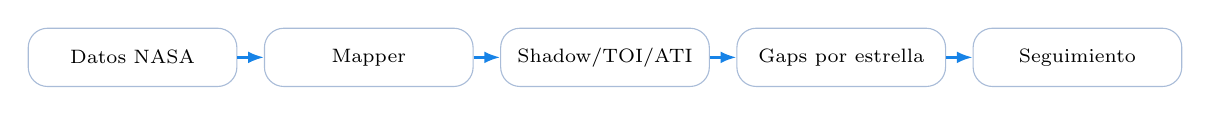
\begin{tikzpicture}[
      pipe/.style={draw=panelline,fill=panel,rounded corners=7pt,minimum width=2.65cm,minimum height=0.74cm,align=center,font=\scriptsize},
      arr/.style={-{Latex[length=2.0mm]},line width=0.85pt,color=accent}
    ]
      \node[pipe] (a) at (0,0) {Datos NASA};
      \node[pipe] (b) at (3.0,0) {Mapper};
      \node[pipe] (c) at (6.0,0) {Shadow/TOI/ATI};
      \node[pipe] (d) at (9.0,0) {Gaps por estrella};
      \node[pipe] (e) at (12.0,0) {Seguimiento};
      \draw[arr] (a)--(b);
      \draw[arr] (b)--(c);
      \draw[arr] (c)--(d);
      \draw[arr] (d)--(e);
    \end{tikzpicture}
  \end{center}
  \vspace{0.08cm}
  \closingbanner{El valor es la capacidad de decidir mejor d\'onde mirar.}
\end{frame}

\begin{frame}[t]{Limitaciones y siguiente trabajo}
  \phasebar{5--6. Evaluation y Communication}
  \vspace{0.10cm}
  \begin{columns}[T,onlytextwidth]
    \begin{column}{0.48\textwidth}
      \infocard{L\'imites}{No reconstruimos el universo completo ni confirmamos planetas faltantes.}
      \vspace{0.08cm}
      \infocard{Dependencias}{Variables elegidas, imputaci\'on, par\'ametros Mapper, proxies de tr\'ansito/RV y calidad de datos del sistema.}
      \vspace{0.08cm}
      \infocard{Sobre estrellas}{Los candidatos intra-sistema son posiciones sint\'eticas de priorizaci\'on, no posiciones confirmadas.}
    \end{column}
    \begin{column}{0.48\textwidth}
      \infocard{Siguiente paso 1}{Injection-recovery por m\'etodo de descubrimiento y por instrumento.}
      \vspace{0.08cm}
      \infocard{Siguiente paso 2}{Funciones de completitud espec\'ificas por estrella, misi\'on y campa\~na.}
      \vspace{0.08cm}
      \infocard{Siguiente paso 3}{TESS, Kepler, Gaia, series RV, N-body e integraci\'on din\'amica.}
    \end{column}
  \end{columns}
\end{frame}

\begin{frame}[plain]
  \astrobackground
  \vspace*{0.92cm}
  {\color{accent}\large\bfseries Cierre}\par
  \vspace{0.28cm}
  {\fontsize{26}{28}\selectfont\bfseries El cat\'alogo de exoplanetas no es el universo planetario.}\par
  \vspace{0.14cm}
  {\fontsize{26}{28}\selectfont\bfseries Es la huella de c\'omo la humanidad lo ha observado.}\par
  \vspace{0.45cm}
  \begin{beamercolorbox}[wd=0.80\linewidth,sep=0.90em,rounded=true]{block body}
    {\small Mapper/TDA permite cartografiar esa huella. TOI/ATI la convierten en prioridad regional. El m\'odulo de estrellas la traduce a intervalos orbitales concretos para seguimiento futuro.}
  \end{beamercolorbox}
  \vfill
  \badge{accentdeep}{universo observable}\hspace{0.08cm}
  \badge{good}{priorizaci\'on interpretable}\hspace{0.08cm}
  \badge{accentdeep}{sistemas estelares}
\end{frame}

\end{document}
